\section{Apparato Sperimentale\footnote{Nota: le indicazioni sulla risoluzione degli strumenti non sono riportate nelle unità di misura del S.I. in quanto abbiamo voluto lasciare le indicazioni sulle modalità di misura dello strumento. Nel seguito della relazione tuttavia tutte le misure effettuate e i risultati trovati saranno espressi nelle opportune unità di misura dell'S.I.}}

\begin{itemize}
	\item{Una bottigla di vetro con un manometro Bourdon di risoluzione di lettura pari a 0.1 bar;}
	\item{Un manometro a U di Torricelli con una risoluzione di lettura di 1 mmHg;}
	\item{Un sistema di raccorderia utilizzato per collegare la pompa a vuoto con la bottiglia;}
	\item{Pompa a mano per raggiungere il basso vuoto;}
	\item{Pompa meccanica a membrana doppio stadio (vuoto limite 500 Pa);}
	\item{Cilindri graduati da 1 \si{\l}, 250 \si{\ml} e 100 \si{\ml} con risoluzione di misura rispettivamente di 10 \si{\ml}, 5 \si{\ml} e 1 \si{\ml};}
	\item{Una bilancia manuale di risoluzione 0.1 g.}
\end{itemize}

\section{Andamento della pressione in funzione del tempo}

Ci proponiamo ora di analizzare l'andamento della pressione interna della bottiglia rispetto a una variabile discreta: il numero di pompate effettuate con la pompa a mano nel primo caso e il tempo nel secondo caso.

\subsection{Acquisizione dei dati}

Le condizioni atmosferiche sono state costanti per tutta la durata dell'esperimento. In particolare la temperatura è stata di 295 $\pm$ 0.5 \si{\kelvin}, una pressione atmosferica di 973 $\pm$ 0.5 hPa e una umidità del 53 $\pm$ 0.5 \%.

\begin{itemize}
	\item{Abbiamo registrato l'andamento della pressione interna alla bottiglia in funzione del numero di pompate effettuate;}
	\item{Abbiamo riempito la bottiglia di aria con un compressore, fino a raggiungere una pressione
	interna di circa a $3 \cdot 10^5$ \si{\Pa}, e abbiamo valutato in funzione del tempo l'andamento della pressione interna alla bottiglia svuotandola con la pompa meccanica a membrana;}
\end{itemize}

\begin{figure}[h!]
    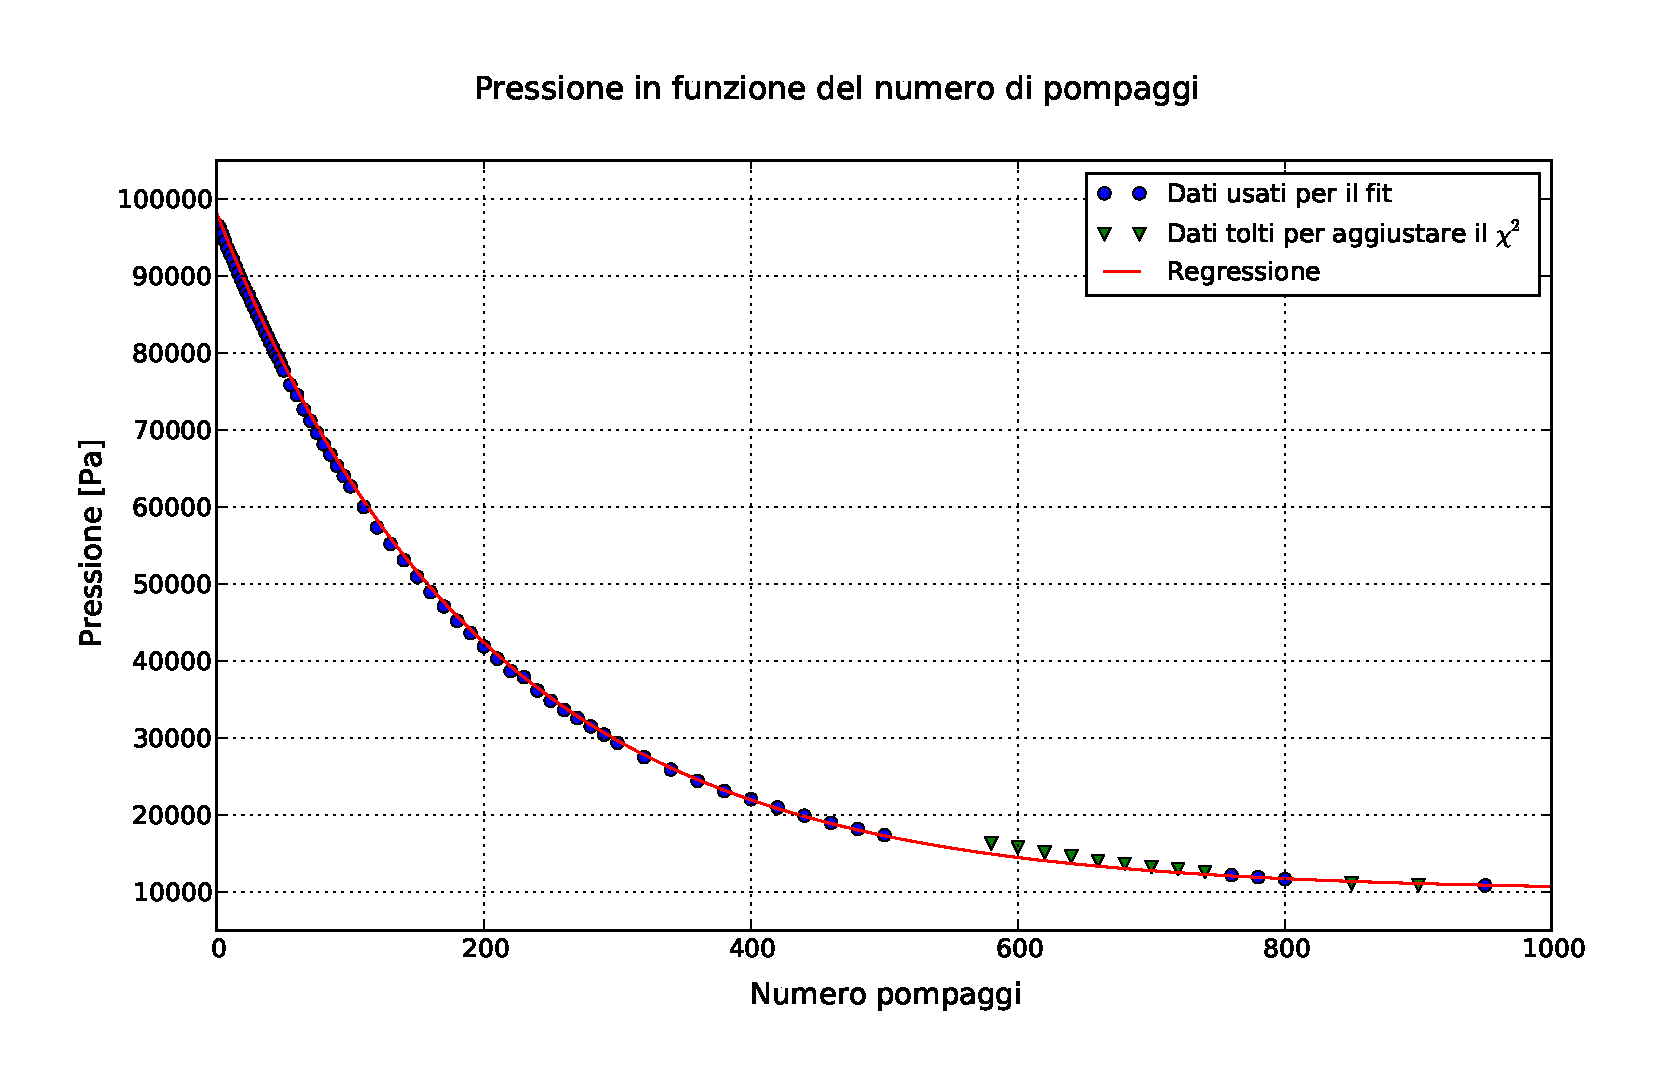
\includegraphics[width=140mm]{graph.pdf}
    \caption{Grafico dei dati ottenuti durante l'esperimento. Il ``buco'' presente tra le 500 e le 580 pompate è dovuto ad una perdita d'aria
    che ci ha costretto a fare 60 pompate per tornare al livello precedente. I punti triangolari sono stati tolti per aggiustare il $\chi^2$.
    Le barre d'errore sono piccole e non visibili. L'andamento riportato è il risultato della regressione.}
    \label{fig:graph1}
\end{figure}

\subsection{Analisi dei dati}

Graficando i dati raccolti relativi all'andamento della pressione in funzione del numero di pompate effettuate otteniamo
il grafico in Figura \ref{fig:graph1}, che come possiamo notare ha un andamento esponenziale. La pressione tende asintoticamente ad un valore di pressione specifico, il vuoto limite della pompa
da noi utilizzata. Tale valore limite è risultato essere, da calcoli numerici di minimizzazzione del chi quadro, di $10080 \pm 50$ \si{\Pa}.

Abbiamo eseguito una regressione, riportata in Figura \ref{fig:graph1}, utilizzando come modello la seguente funzione:

\begin{equation}
    P = P_{0(1)} e^{-an} + P_{l(1)}
\end{equation}
%
dove n è il numero di pompaggi, $P_{0(1)}$ e $a$ sono costanti e $P_{l(1)}$ indica la pressione limite.

Con il metodo dei minimi quadrati abbiamo ottenuto i valori:
\begin{equation}
    P_{0(1)} = 97990 \pm 50 \; \si{\Pa} \qquad a = (5.014 \pm 0.006) \cdot 10^{-3} \qquad P_{l(1)} = 10080 \pm 50\; \si{\Pa}
\end{equation}

Come si vede dal grafico in Figura \ref{fig:graph1},
durante l'esperimento si è verificata una perdita attorno alla 500-esima pompata, che ci ha costretto a scartare alcuni punti.
Comunque abbiamo ottenuto un valore di $P_{0(1)}$ %CORREGGERE {l(1)}$
di poco differente dal valore misurato di $97330 \pm 50 \; \si{\Pa}$.
L'incompatibilità tra i due valori può essere dovuta alla perdita d'aria che ha guastato i nostri dati.

Il grafico dell'andamento della pressione in funzione del tempo trascorso dall'inizio del processo di svuotamento della bottiglia da parte della pompa meccanica a membrana è riportato in Figura \ref{fig:graph2}. Si può notare la somiglianza con il grafico in Figura \ref{fig:graph1}. I punti sperimentali seguono la stessa legge esponenziale. L'esponenziale in figura è quello ottenuto della regressione lineare
\begin{equation}
    P = P_{0(2)} e^{-bt} + P_{l(2)}
\end{equation}
dove $t$ è il tempo, P$_{0(2)}$ e $b$ sono costanti e $P_{l(2)}$ è la pressione limite:
\begin{equation}
    P_{0(2)} = 87700 \pm 500 \; \si{\Pa} \qquad b = 0.164 \pm 0.001 \qquad P_{l(2)} = 4000 \pm 1200 \; \si{\Pa}
\end{equation}

\begin{figure}[h!]
    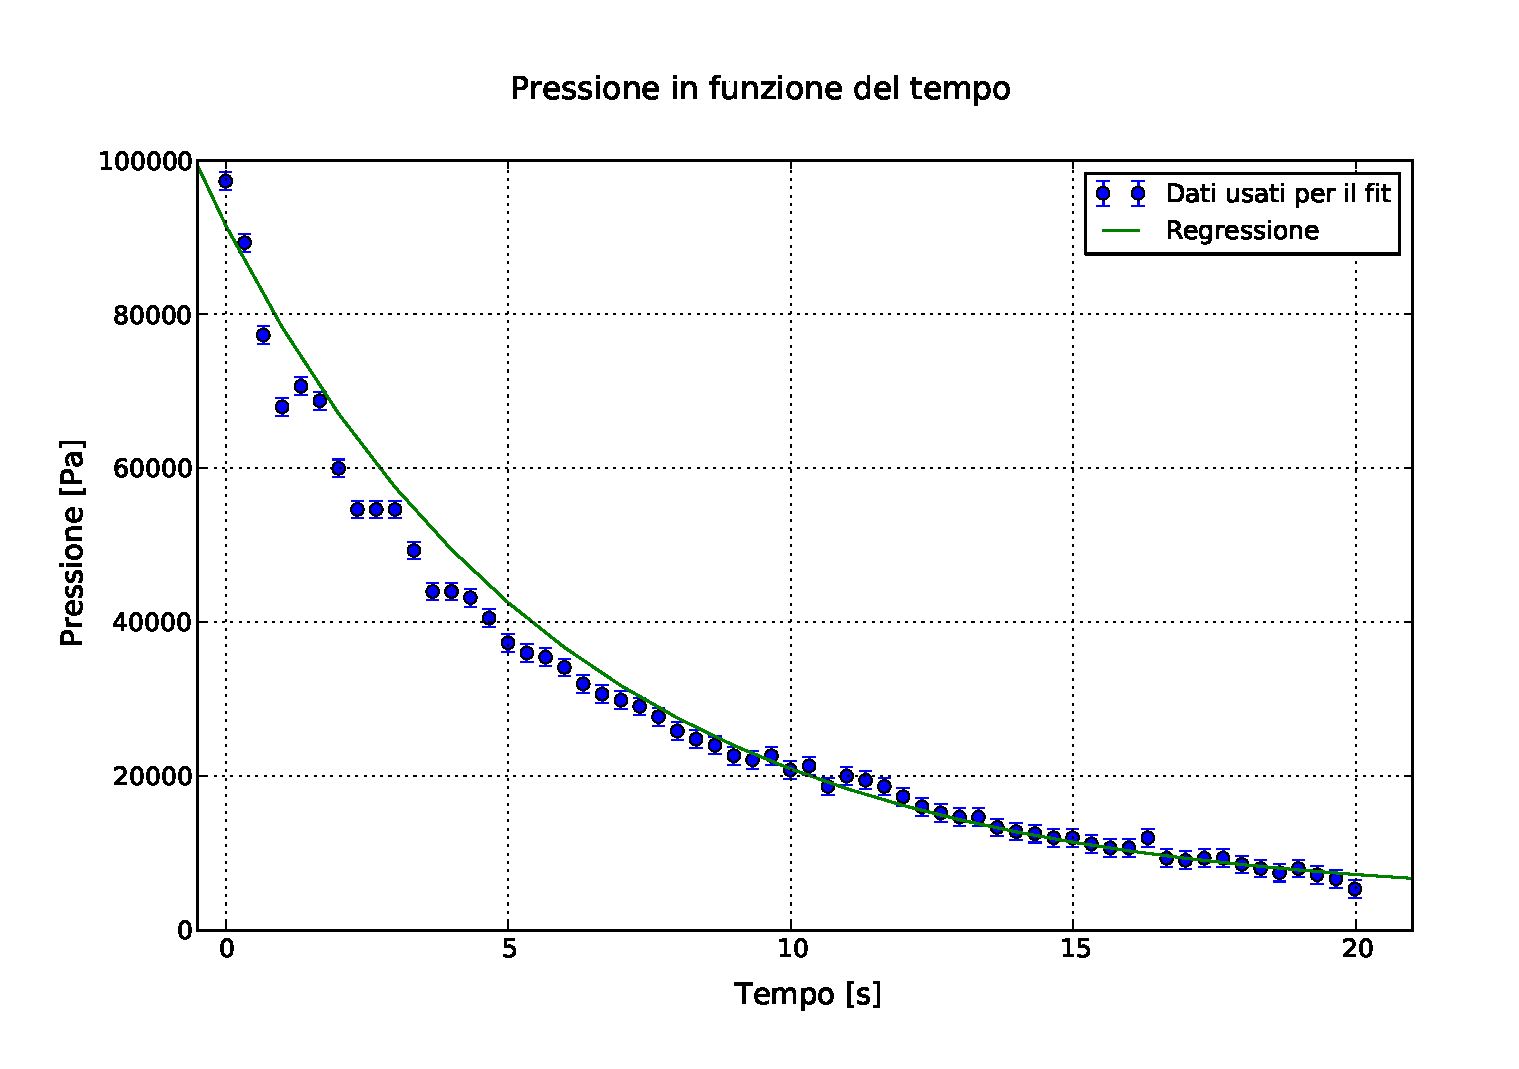
\includegraphics[width=140mm]{graph2.pdf}
    \caption{Il grafico mostra la pressione in funzione del tempo ricavata dal video della pompa a membrana. I dati sono di scarsa qualità, l'errore è molto alto
	ed il fit non segue molto bene i dati. Purtroppo con i dati in nostro possesso non siamo riusciti a fare di meglio.}
    \label{fig:graph2}
\end{figure}
